% This is samplepaper.tex, a sample chapter demonstrating the
% LLNCS macro package for Springer Computer Science proceedings;
% Version 2.20 of 2017/10/04
%
\documentclass[runningheads]{llncs}
% 
\usepackage{hyperref}
\usepackage{graphicx}
\usepackage{tabularx}


% Used for displaying a sample figure. If possible, figure files should
% be included in EPS format.
%
% If you use the hyperref package, please uncomment the following line
% to display URLs in blue roman font according to Springer's eBook style:
%\renewcommand\UrlFont{\color{blue}\rmfamily}

\begin{document}
%
\title{Challenge 1: Mars Rover}
%
%\titlerunning{Abbreviated paper title}
% If the paper title is too long for the running head, you can set
% an abbreviated paper title heres
%
\author{Fernando Alcántara \and
Arturo Burela \and
Horacio Rojas}
%
\authorrunning{F. Author et al.}
% First names are abbreviated in the running head.
% If there are more than two authors, 'et al.' is used.
%
\institute{Instituto Tecnológico y de Estudios Superiores de Monterrey}
%
\maketitle              % typeset the header of the contribution
%
\begin{abstract}
The present paper will explore how reactive agents work, the main characteristics of reactive agents and a comparison between individual and collaborative behaviour,
all of the above through a couple of simulations of the Mars explorer problem (Weiss, 1999) and a performance analysis of the scenarios.

\keywords{Multi Agent System  \and Distributed Artificial Intelligence \and Reactive Agents.}
\end{abstract}
%
%
%
\section{First Section}
\subsection{Introduction}

Agents are often described as entities that perceive, reason, act and communicate. Reactive agents are a subset of agents, some characteristics of reactive agents are simplicity and flexibility. Reactive agents don't use models of the environment, they only use immediate information available and they do not carry out deliberative processes such as learning. However, reactive agents are really effective for simple tasks and don't require much compute power making them useful for reaction mechanisms and short term activities.

Reactive agents are not intelligent, they do not have any knowledge representation so they can not perform reasoning or learning. Nevertheless a good rule set will provide any agent good capability to solve simple to medium complex tasks. Rule sets define agents actions according to environment perception and are the only logic within a reactive agent, each rule has a different hierarchy and the whole set determines the actions to take in every situation.

Multi agent systems are systems where two or more agents interact with each other and the environment, that means that even not knowledge based agents (as reactive agents) are capable to form a working multi agent system if they are conceived with the correct configuration. In the following sections different simulations are done to demonstrate that reactive agents can accomplish tasks effectively, especially when using multiple agents capable of communicating between them.

\section{Second Section}
\subsection{Apparatus}

The apparatus consists of a simulation of the Mars explorer problem (Weiss, 1999). This problem describes a situation where robot explorers in Mars are given the task of collecting Martian rocks and return them to the base. Each robot has a limited load capacity and therefore they need to return to the base when they can't carry more rocks. The simulation ends when all rocks (or a specific number) are collected.

For this challenge we decided to build our own simulator based on web technologies, both to make it more visually appealing and to use it in the future. The simulation was build with ThreeJS, a WebGL JavaScript library capable of loading full 3D scenes in the browser leveraging the GPU of the computer. All agents logic, environment initial configuration, and simulation results are built using JavaScript.

The environment consist of the surface of Mars, the Martian base and multiple obstacles in the terrain. Targets (rocks) and obstacles (UFOs) are instantiated randomly over the surface every iteration of the simulation. The agents always start near the base and they consist of a Mars rover robots capable of moving freely by the terrain except by obstacles.

Two different simulations were made, both with the same number of agents, targets and obstacles. The first one is a reactive multi agent system, with 6 agents on the surface collecting rocks, each of them running the same rule set. The second simulation has the same number agents, targets and obstacles but the rule set of the agents is different because agents are now able to communicate to each other and they perceive others position in the scene. Each simulation was ran multiple times, both setups were tested with randomly positioned targets and obstacles every iteration.

\section{Third Section}
\subsection{Behaviours \& Experiments}

Each simulation was done 100 times, we took statistics of every iteration and using that data we compared the performance of the two scenarios. The following results reveal insights of the difference between a slightly different implementation of reactive agents.

\subsubsection{Multi Agent System}

On this simulation agents were uncommunicated, they all had the same goal of collecting rocks but were exploring and carrying all by themselves. This behaviour accomplished the task but was slow and inefficient, most robots visited the same area twice without finding new rocks.

\begin{figure}[htp]
\centering
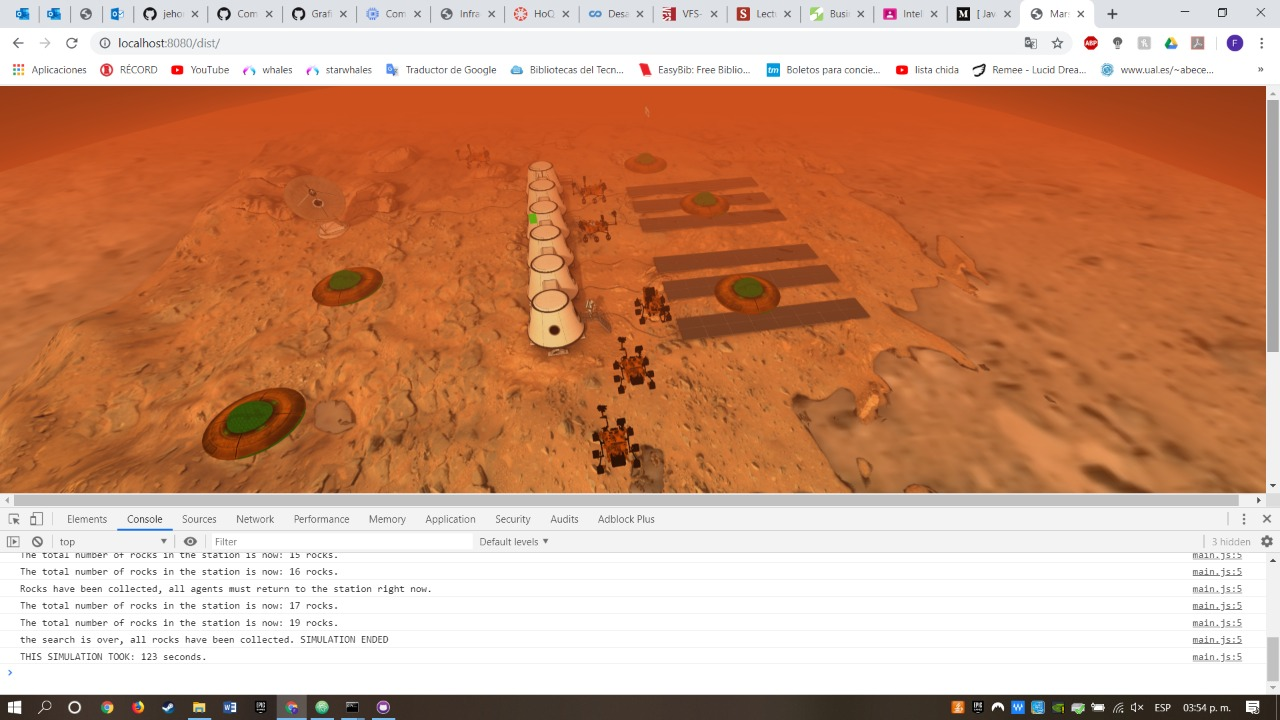
\includegraphics[width=\textwidth,height=\textheight,keepaspectratio]{result.jpeg}
\caption{Simulation 1}
\label{Final state screenshot of the simulation}
\end{figure}

\begin{center}

\begin{tabularx}{\textwidth}{X|l}
  \textbf{Performance Metric} & \textbf{Result average} \\
\hline
Solution time: Total time to collect all rocks & 125 seconds\\
Robot Effectiveness: Rocks collected per robot & 0.81 rocks\\
Robot Efficiency: Obstacle hits per robot & 5.67 hits\\
Robot Efficiency: Covered distance per robot & 198.12 units\\
\end{tabularx}
\end{center}



\subsubsection{Multi Agent System with Communication} 
This simulation performed way better that the no communication variant, finish time was reduced by almost 50\% and each robot carried at least 1 rock in every simulation increasing resource (robots) utilization efficiency almost 2 times. With synchronized rocks discovery and position reporting robots needed to travel less to cover more area and pick more rocks.


\begin{figure}[htp]
\centering
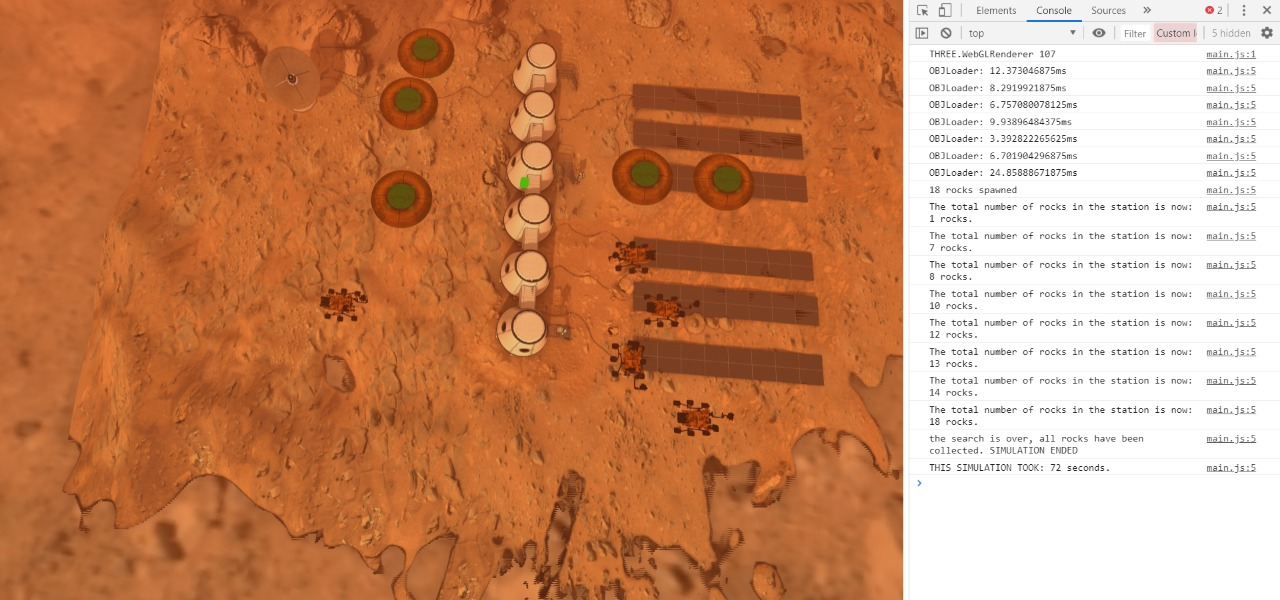
\includegraphics[width=\textwidth,height=\textheight,keepaspectratio]{result2.jpeg}
\caption{Simulation 2}
\label{Final state screenshot of the simulation}
\end{figure}

\begin{center}
\begin{tabularx}{\textwidth}{X|l}
  \textbf{Performance Metric} & \textbf{Result average} \\
\hline
Solution time: Total time to collect all rocks & 74.34 seconds\\
Robot Effectiveness: Rocks collected per robot & 1.56 rocks\\
Robot Efficiency: Obstacle hits per robot & 4.89 hits\\
Robot Efficiency: Covered distance per robot & 138.24 units\\
\end{tabularx}
\end{center}


\section{Fourth Section}
\subsection{Conclusions}
After comparing the performance of both simulations we came with 3 different ideas. The first one is that even if reactive agents may seem old and not quite intelligent they are still useful to solve small to medium sized problems, especially if we don't have many historic data of the problem to build knowledge. This means that sometimes simple approaches as reactive agents are good enough to tackle simple problems, otherwise using machine learning or other more sophisticated methods may result costlier and slower.

Second, we determined the importance of rule sets and rules hierarchy, by variation of both rules actions and rules hierarchy we were able to make agents perform better and take better actions according to the situation.

Finally, we learned the importance of communication and environment perception. Even with rule variation the performance gains were not as big as when communication was introduced. Communication between agents permitted more organized work and also more environment perception in less time, this information transfer between agents make each one take better actions using practically the same rule set.

\section{Manual}
The following section describes how to visualize and use the simulation. As this program is web based the user only need to have a modern browser compatible with JavaScript ES5 / ES6 and WebGL (WebGL 2 is recommended).
ThreeJS has dependencies that may limit browser support, however WebGL is the principal requirement, Google Chrome 9+, Firefox 4+, Opera 15+, Safari 5.1+, Internet Explorer 11 and Microsoft Edge are compatible. You can find which browsers support WebGL at \href{https://caniuse.com/\#feat=webgl}{Can I use WebGL}.

To use the simulator access the following URL: \url{https://arturoburela.github.io/IntelligentSystems/MarsRover/} with a compatible browser. The scene may take a couple of seconds to load, after the initial load you should see the 3D environment of the simulation. On the browser console you can see some logs of the simulation performance. The source code of the project is available at \url{https://github.com/ArturoBurela/IntelligentSystems/tree/master/Activity1-MarsRover/src}.
%
% ---- Bibliography ----
%
% BibTeX users should specify bibliography style 'splncs04'.
% References will then be sorted and formatted in the correct style.
%
% \bibliographystyle{splncs04}
% \bibliography{mybibliography}
%
\begin{thebibliography}{8}

\bibitem{ref_url1}
ThreeJS, \url{https://threejs.org/}. Last accessed 14
September 2019
\bibitem{ref_url2}Weiss, G. (1999). Multiagent systems: a modern approach to distributed artificial intelligence. Estados Unidos: The MIT Press.
\url{http://uma.ac.ir/files/site1/a_akbari_994c8e8/gerhard_weiss___multiagent_systems___a_modern_approach_to_distributed_artificial_intelligence.pdf}. Last accessed 14
\bibitem{ref_url3}
Vlassis, N. (2003). A Concise Introduction to Multiagent Systems and Distributed AI. septiembre 15, 2019, de Universidad de Amsterdam, \url{http://citeseerx.ist.psu.edu/viewdoc/download?doi=10.1.1.335.1794&rep=rep1&type=pdf}. Last accessed 14
September 2019
\end{thebibliography}
\end{document}
